%Chapter 3

\renewcommand{\thechapter}{6}

\chapter{Additional Contributions}

During my time at the University of Maryland, I have had the privilege to work on a wide array of interesting problems in key areas of bioinformatics.
The ever-increasing amount of sequencing data poses a challenge to commodity hardware both in terms of storage and analysis.
In this chapter, I describe my contributions to the fields of lossy compression and clustering.
In Section \ref{lossy-section}, I show how that we can use lossy compression algorithms to greatly reduce the required storage for next generation sequencing data with little effect on downstream analyses.
In Section \ref{kmulus-section}, I show how we can leverage the power of cloud computing to cluster sequencing data and speedup sequence alignment.
I mentored two undergraduate students to complete this project.

\section{Lossy Compression of DNA Sequence Quality Values}
\label{lossy-section}
\subsection{Abstract}


The \textsc{fastq} file format has become the \emph{de facto} standard
for storing next-generation sequencing data, containing nucleotide
information along with a quantitative measure of the reliability of
individual base calls. As the cost of sequencing continues to
decrease, the rate of sequencing data production is increasing,
requiring efficient ways of storing and transferring this vast amount
of data. Most methods on sequencing data compression focus on
compressing nucleotide information without any loss of information.
Quality data, however, have different properties than nucleotide data,
and methods compressing nucleotide sequences efficiently do not
perform as well on quality sequences. Furthermore, while lossless
representation is necessary for nucleotide sequences, it is not an
essential requirement for quality values.

Existing methods for compressing quality sequences mostly focused on
minimizing the loss of information with less emphasis on effects on
subsequent analyses. In this chapter, we evaluate several different
compression methods for quality values that compromise accuracy for
better storage efficiency, and their resulting impact on common
bioinformatic analyses using sequence read data.

Lossy compression of quality information can greatly decrease storage
and memory requirements with little discernible effects on subsequent
analysis results. The three compression strategies in this study were
able to produce similar results to those obtained with uncompressed
quality sequences in terms of quality control, genome assembly, and
alignment of short read to a reference sequence.

\subsection{Introduction}

Read data from high-throughput sequencing constitutes the largest
category of data in genomics research because of great redundancy,
inclusion of quality values, and read-level naming and
metadata. Because of this abundance effective compression of read data
has the potential for substantial improvement in data storage and
transfer efficiency.

Quality values comprise a standard component of \textsc{fastq}
files~\cite{Cock:2010ve}, a very common format for sequence read
data. At the level of sequence read the probability of error for each
base-call is typically represented by \textsc{phred} quality value,
which is defined as $Q =
-10\,log_{10}P$~\cite{Ewing:1998ly}. Depending on the sequencing
technology these quality values can range from 0 to 93, and are
represented with the \textsc{ascii} characters 33 to 126 (with some
offset). There is a single quality value per base-call for Illumina
sequence reads.

Quality values can be used throughout bioinformatics pipelines. Among
the most fundamental uses of sequence quality values is as part of the
quality assessment and quality control (\textsc{qa/qc}) processes
prior to subsequent analysis steps. Quality control based on quality
values generally includes two operations: \textit{i}.~filtering, the
elimination of reads that on the whole do not meet arbitrary quality
standards, which reduces the total number of reads; and
\textit{ii}.~trimming of low quality base-calls from reads, which
reduces the number total number of bases. Quality values can be used
by genome assembly software to produce better
assemblies~\cite{Bryant:2009uq,Gnerre:2011kx}. Short-read
alignment software, such as Bowtie2~\cite{langmead2012fast}, use
quality values to weight mismatches between read and reference
sequences. Software for detecting single nucleotide polymorphisms
(\textsc{snp}s) can use quality values~\cite{McKenna:2010bh},
and identified \textsc{snp}s with high-quality calls are deemed more
reliable than those with low-quality calls, particularly in low
coverage regions.

Previous literature on sequence data compression has largely focused
on lossless compression of base calls~\cite{asnani2012lossy,Canovas:2014fr,Hach:2012ys,
  janin2013adaptive,Kozanitis:2011kl,Ochoa:2013rt,Tembe:2010ys,
  Wan:2012kq,DBLP:conf/recomb/YuYB14,zhou2014compression}. Among the
several challenges for compression of read data is dealing with
different error profiles resulting from differences in underlying
chemistries, signal detection and processing mechanisms, inherent
biases, and other idiosyncratic properties of distinct high-throughput
sequencing technologies. Sequence reads generated by instruments such
as an Illumina HiSeq, the focus of this research, are characterized by
having relatively few insertion and deletion errors, but substitution
(miscall) errors are much more frequent and have context-specific
patterns. These errors are non-uniformly distributed over the read
length (e.g., error rates increase up to $\sim$16$\times$ at the
3$^{\prime}$ end, and 32.8 -- 67.9\% of reads have low quality tails
at the 3$^{\prime}$ end~\cite{Minoche:2011km}).

Although we recognize the need for lossless compression for some
purposes and contexts (e.g., archiving, provenance), our perspective
is largely pragmatic with a focus on the use of quality values in
subsequent analyses. From this perspective some loss of information is
deemed acceptable if the inferences from analyses are relatively
unaffected. Here we describe our research investigating lossy
compression of sequence read quality values, specifically those
associated with Illumina instruments, with the objective to provide
some perspective on several strategies rather than to develop a robust
high-quality software for use. Recognizing these properties of
Illumina sequence reads motivates our exploration of three general
classes of lossy compression methods -- binning, modeling, and
profiling -- and consider an exemplar of each class.~\cite{Canovas:2014fr} and~\cite{janin2013adaptive} evaluated the effects of lossy compression on identifying variants within a dataset. We build on these prior works and access the effects of
% quantifying compression efficiency, we also assess the effects of
quality value information loss resulting from compression on additional
subsequent genomic analyses including read preprocessing (filtering
and trimming), genome assembly, and read mapping.

\subsection{Methods}

\subsubsection{Compression strategy: binning}

Quality values can be binned, and the minimum number of bins that
allows for a any distinction among quality values is two, i.e., two
categories ``good'' and ``bad'' quality. We implement 2-bin encoding
by setting a quality value threshold empirically determined by the
distribution of quality values across reads. Base-calls are marked
``bad'' if their quality value falls below the first quartile minus
1.5 $\times$ the interquartile range (IQR), which is the difference
between the first and third quartile. 1.5 $\times$ IQR is the value
used by Tukey's box plot~\cite{mcgill1978variations}. The main
benefit of this approach is that it is completely data-dependent, and
no assumptions regarding the distribution of the quality values need
to be made.

With 2-bin encoding binary encoding is possible, allowing us to use a
single bit to represent the quality of a base instead of the standard
8 bits used to store quality values in \textsc{ascii}. An additional
benefit of 2-bin encoding is the potential for increased adjacency of
identical values and repeating patterns, properties that may increase
effectiveness of subsequent compression using established
algorithms~\cite{HUFFMAN:1952nr,Ziv77auniversal,
  DBLP:journals/tit/ZivL78}.

The economic costs of memory use for binning, in general terms,
include no fixed costs, and marginal costs that are a function of the
number of base-call quality values times the cost of the encoding.

\cite{Wan:2012kq} provide three similar lossy compression strategies based on binning the base error probability distribution: UniBinning, Truncating, and LogBinning.
UniBinning evenly splits the error probability distribution into a user-defined number of partitions.
Truncating treats a user-defined number of highest quality values as a single bin.
LogBinning works similar to UniBinning, except with the \emph{log} of the error probability distribution, which effectively bins the \textsc{ascii} quality values evenly.
Our 2-bin encoding is a combination of LogBinning and Truncating in that we are placing the highest quality values (as defined above) of the log of the error probability distribution into a single bin.


\begin{figure}[!tpb]%figure2
\begin{center}
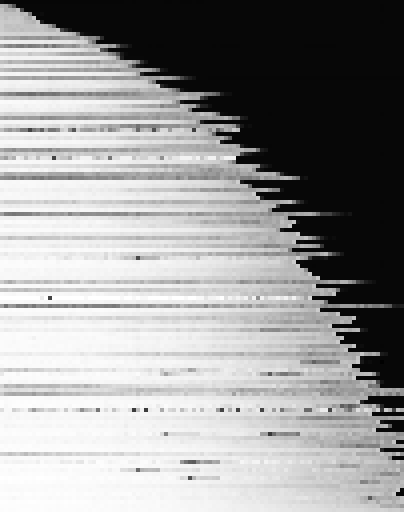
\includegraphics[width=.9\textwidth]{profiles_128.png}
\end{center}
\renewcommand{\baselinestretch}{1}
\small\normalsize
\begin{quote}
\caption[Quality profiles obtained by $k$-means clustering on the
  fragment library from \textit{Rhodobacter sphaeroides} 2.4.1 data
  set]{Quality profiles obtained by $k$-means clustering on the
  fragment library from \textit{Rhodobacter sphaeroides} 2.4.1 data
  set using $k$ = 128, with each row corresponding to a quality
  profile. Dark to light colors represent low to high quality
  values. It is readily visible that the two most distinctive features
  of quality profiles is their drop-off position and average overall
  quality. One can also see sporadic low-position values in a handful
  of profiles, likely capturing intermittent problems in the
  sequencing process affecting thousands of reads at a
  time.}
  \label{fig:profiles_128}
\end{quote}
\end{figure}
\renewcommand{\baselinestretch}{2}
\small\normalsize

\subsubsection{Compression strategy: modeling}

If quality values are modeled, compression is conceivably possible by
replacing the original quality values by a representation of the
model. For example, quality values can be conceptualized as bivariate
data with the ordered nucleotides (1 to read length) representing the
abscissa, and quality values representing the ordinate. In this
research we model read quality values as polynomial functions obtained
with least-squares fitting, as one approach to compression read
quality values by modeling.

Despite the fact that polynomial functions have significantly lower
number of parameters (i.e. one to six coefficients) than a read-length
string of raw quality values, the necessity of using floating point
numbers to store coefficients greatly limits the compression potential
of the method. In order to get meaningful compression on
single-precision four-byte floating point numbers, one would have to
relax on the least-squares approximation constraint to obtain
compressible values on the byte level which is outside the scope of
this study.

The economic costs of memory use for model-based compression, in
general terms, include no fixed costs, and marginal costs that are a
function of the number of reads times the cost representing the model
parameters.

\textsc{QualComp} is a lossy compression tool that models quality values as a multivariate Gaussian distribution, computing the mean and covariance for each position in the read\cite{Ochoa:2013rt}.
Once the model parameters are calculated, they are stored by the decoder to later reconstruct a \emph{representative} quality value.
\textsc{QualComp} takes as input a user-specified rate (bits per read) and then poses an optimization problem of how to allot these bits for a given position while minimizing the \textsc{mse}.
The quality values can be clustered before hand to produce more accurate models.

\subsubsection{Compression strategy: profiling}

As large sets of quality strings show similar trends of quality over
their length, it makes sense to identify such common patterns in the
data and use them as reference profiles to approximate individual
sequences of quality values. Such patterns can be readily determined by
clustering data points (i.e. quality vectors) and using the resulting
cluster centers as representative profiles.

$k$-means clustering is a vector quantization method, partitioning a
set of samples into $k$ sets that minimize within-cluster sum of
squares~\cite{macqueen1967some}. Using a random subset of read
quality values, a compression method can use the computed cluster
centers as read quality profiles. As the problem is NP-hard, we use a
heuristic iterative refinement approach by quickly converging to a
locally optimal minimum provided by R~\cite{hartigan1979algorithm}.

First, the method samples an adjustable number of reads
randomly from the file to be used as a training set. Quality values
are represented by vectors containing their \textsc{phred} scores
corresponding to each position along the read. Subsequently, $k$-means
clustering is performed on the training set until convergence. The
obtained cluster centers will be the quality profile prototypes for
the dataset.

Once the $k$ quality profiles are determined, all reads
are passed through the trained $k$-means predictor, with the nearest
quality profile in Euclidean space being assigned to every read
as their compressed representation.

The compressed quality file therefore consists of an index enumerating
the $k$ quality profiles, and a binary part containing the assigned
quality profile index for each read.

Although this approach is not able to capture randomly occurring
outlier quality values, it ensures that the overall trends in quality
value patterns are retained. Quality profiles capture different overall
qualities and different drop-off positions and gradients. An example
of 128 quality profiles are shown on Figure \ref{fig:profiles_128}.

The economic costs of memory use for profile-based compression, in
general terms, include fixed costs associated with representing the
profiles, which is a function of the number of profiles times the cost
of encoding them, and these fixed costs are amortized over the entire
set of reads to which they apply. Additionally there are marginal
costs that are a function of the number of reads encoded.

\subsubsection{Datasets}

We used several Illumina sequence read datasets in this research,
which are taken from data from the \textsc{gage} (Genome Assembly
Gold-Standard Evaluations)~\cite{Salzberg:2012rc} except as
noted. These datasets are as follows.

\textit{Rhodobacter sphaeroides} 2.4.1, which are generated from a
fragment library (insert size of 180 nt; 2,050,868 paired-end reads)
and short-jump library (insert size of 3,500 nt; 2,050,868 reads). The
corresponding reference sequence was obtained from the NCBI RefSeq
database (NC\_007488.1, NC\_007489.1, NC\_007490.1, NC\_007493.1,
NC\_007494.1, NC\_009007.1, NC\_009008.1).

% Will be moved to supplemental.
%\textit{Stapylococcus aureus} USA300, which are generated from a
%fragment library (insert size of 180 nt; 1,294,104 paired-end reads)
%and short-jump library (insert size of 3,500 nt; 3,494,070 reads).
%The corresponding reference sequence was obtained from the NCBI RefSeq
%database (NC\_010063.1, NC\_010079.1, NC\_012417.1).

\textit{Homo sapiens} chromosome 14 data, which are generated from a
fragment library (insert size of 155 nt; 36,504,800 paired-end reads)
and short-jump library (insert sizes ranging from 2283-2803 nt;
22,669,408 reads). The corresponding reference sequence was obtained
from the NCBI RefSeq database (NC\_000014.8).

\textit{Escherichia coli} str. K-12 MG1655 MiSeq data was downloaded
from \url{http://www.illumina.com/systems/miseq/scientific_data.html},
which are generated from a fragment library (insert size of 180 nt;
1,145,8940 paired-end reads). The corresponding reference sequence
was obtained from the NCBI RefSeq database (NC\_000913.2).

\textit{Mus musculus} data was downloaded from
\url{http://trace.ddbj.nig.ac.jp/DRASearch/run?acc=SRR032209}, which
consisted of 18,828,274 reads of length 36.


% \begin{landscape}
% \renewcommand{\baselinestretch}{1}
% \small\normalsize
% \begin{quote}
% \begin{figure}
% \begin{center}
% 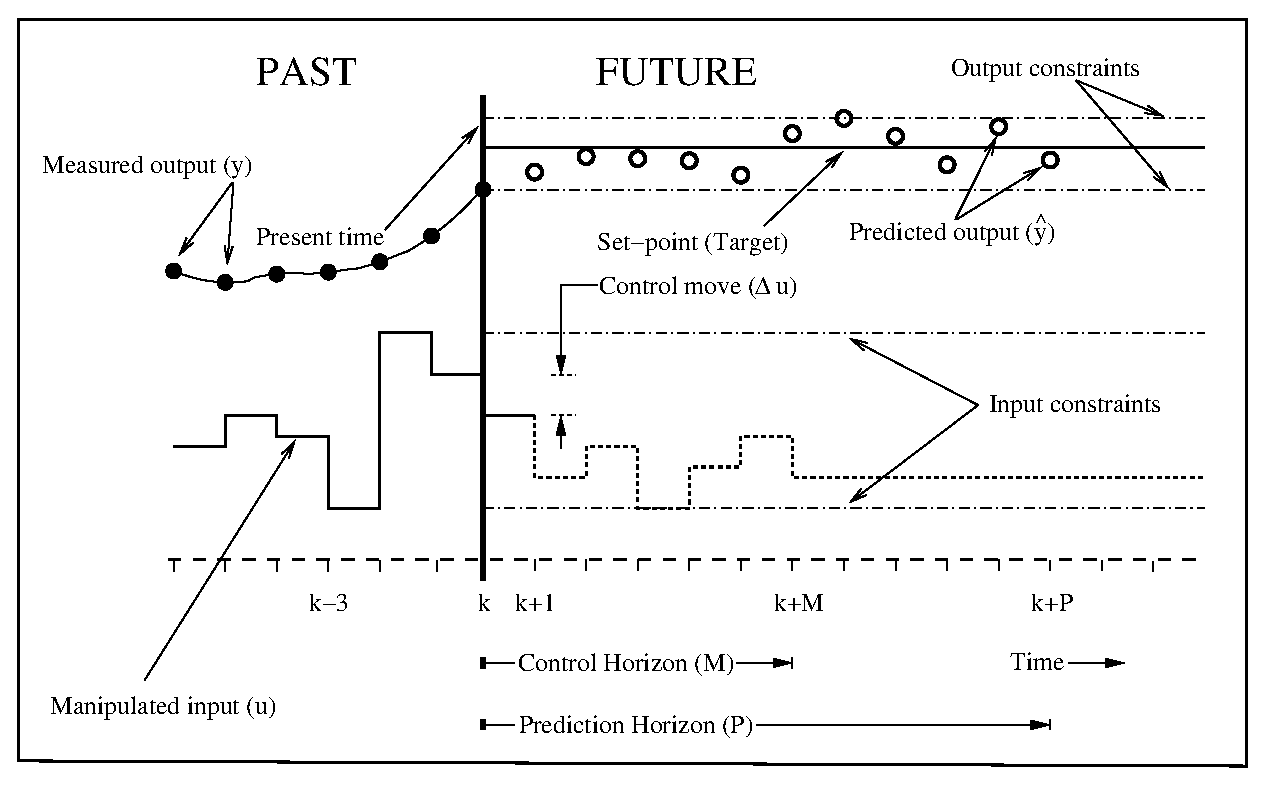
\includegraphics[width=8.2in]{mpc.eps}
% \end{center}
% \caption{Schematic illustrating receding horizon control.
% \label{fig:mpc} }
% \end{figure}
% \end{quote}
% \renewcommand{\baselinestretch}{2}
% \small\normalsize
% \end{landscape}

\subsubsection{Performance evaluation}

As a measure of compression effectiveness we use bits/base-call, and
define it as the size of the compressed representation of quality
values (in bits) divided by the number of quality values represented.
As a measure of information loss we use mean squared error
(\textsc{mse}) as a loss function, and define it as
$\frac{1}{n}\sum_{i=1}^{n}{(Q_i'-Q_i)^2}$, where $n$ is the number of
sequences, $Q_i'$ is the compressed/decompressed quality value, and
$Q_i$ is the original quality value associated with sequence position
$i$.

We evaluate effects of information loss from quality value compression
on quality control steps of read filtering and trimming, which were
performed using Sickle~\cite{sickle}, and make comparison to
uncompressed data.

We evaluate effects of information loss from quality value compression
on \emph{de novo} genome assembly performance using contiguity
statistics, log average read probability
(\textsc{lap})~\cite{LAP}, and a collection of
reference-based metrics. The contiguity statistics include N50, which is defined as the median contig
size (the length of largest contig $c$ such that the total size of the
contigs larger than $c$ exceeds half of the assembly size) and corrected N50, which is the recalculated N50 size after the contigs are broken apart at locations of errors. The
\textsc{lap} score can be viewed as a log likelihood score, where a
value closer to 0 is better. We use a script provided by \textsc{gage}
reference-based evaluation to count single nucleotide polymorphisms
(\textsc{snp}s), relocations, translations, and inversions. The
reference-based metrics are normalized by the length of the assembly
to facilitate comparison. For the genome assembly we used software
that makes use quality values in the assembly process:
\textsc{allpaths-lg}~\cite{Gnerre:2011kx} version r50191 with default
settings and 32 threads.

\subsection{Results}

\subsubsection{Compression effectiveness versus information loss}

We compare the \textsc{mse} versus bits/base-call of the
\textit{Rhodobacter sphaeroides} 2.4.1, \textit{Homo sapiens}
chromosome 14, \textit{Escherichia coli} str. K-12 MG1655, and
\textit{Mus musculus} datasets (Figure \ref{fig:mse_vs_bpbp}). We
only include the fragment libraries for the \textit{Rhodobacter
  sphaeroides} 2.4.1, and \textit{Homo sapiens} chromosome 14 data
sets, but the additional short-jump library results are available in
the Supplementary of the submitted manuscript. Storing the uncompressed quality
values requires 1 byte per base-call because they are stored in
\textsc{ascii} format and is denoted by the dotted black asterisk in
the figure. The lossless compression of each dataset using \textsc{bz}ip2
ranges from 2.19 - 3.10 bits/base-call and is denoted by the colored
asterisks on the abscissa. The compression methods tend to cluster
together across the different datasets. Across all datasets, the
0-degree polynomial regression, profile encodings, and \textsc{q}ual\textsc{c}omp have
the lowest bits/base-call.


\begin{landscape}
\renewcommand{\baselinestretch}{1}
\small\normalsize
\begin{quote}
\begin{figure}[!tpb]%figure2
\begin{center}
\includegraphics[width=1.4\textheight]{compression_results.pdf}
\end{center}
\renewcommand{\baselinestretch}{1}
\small\normalsize
%\begin{quote}
\caption[Mean squared error versus bits/base-call for different
  compression methods applied to the \textit{Rhodobacter sphaeroides}
  2.4.1, and \textit{Homo sapiens} chromosome 14 fragment libraries,
  and \textit{Escherichia coli} str. K-12 MG1655, and \textit{Mus
    musculus} datasets]{Mean squared error versus bits/base-call for different
  compression methods applied to the \textit{Rhodobacter sphaeroides}
  2.4.1, and \textit{Homo sapiens} chromosome 14 fragment libraries,
  and \textit{Escherichia coli} str. K-12 MG1655, and \textit{Mus
    musculus} datasets. 2B --- 2-bin encoding; P$n$ --- profiling
  with $n$ profiles; R$n$ --- modeling with polynomial regression
  models of degree $n$; Q$n$ --- \textsc{q}ual\textsc{c}omp with rate parameter of
  $n$. Asterisks denote the corresponding lossless compression using
  \textsc{bz}ip2, with the black asterisk corresponds to original uncompressed
  data.}
  \label{fig:mse_vs_bpbp}
\end{figure}
\end{quote}
\renewcommand{\baselinestretch}{2}
\small\normalsize
\end{landscape}


\textsc{q}ual\textsc{c}omp with the rate parameter set to 100 bits/read has the lowest
\textsc{mse}, but requires 10-15x more storage than the profile
encoding methods for only a 2-3x reduction in \textsc{mse}. When
\textsc{q}ual\textsc{c}omp's rate parameter is set to match the profile encoding
methods, \textsc{q}ual\textsc{c}omp performs slightly worse in terms of \textsc{mse}.
In the \textit{Rhodobacter sphaeroides} 2.4.1 fragment library,
\textsc{q}ual\textsc{c}omp with rate 10 bits/read (0.099 bits/bp) has a \textsc{mse} of
17.29. Using 256-profile encoding requires less storage (0.079
bits/bp) and has a lower \textsc{mse} (11.85).

As the order of the polynomial increases, the bits/base-call increase
and the \textsc{mse} decreases at an exponential rate. The 7th-degree
polynomial regression has the highest bits/base-call and in the
\textit{Mus musculus} dataset, and requires more storage than the
\textsc{ascii} original quality values. A 7th-degree polynomial
requires storing eight floating point values, resulting in 32 bytes
per sequence of quality values. The read length of the \textit{Mus musculus}
dataset is only 26, so the 7th-degree polynomial regression is storing
six more bytes than necessary for lossless encoding the quality data.

\begin{figure}[!htb]%figure2
\begin{center}
\includegraphics[width=4in]{preprocessing_results.pdf}
\end{center}
\renewcommand{\baselinestretch}{1}
\small\normalsize
\begin{quote}
\caption[Preprocessing results of \textit{Rhodobacter sphaeroides}
  2.4.1, and \textit{Homo sapiens} chromosome 14 fragment libraries,
  and \textit{Escherichia coli} str. K-12 MG1655, and \textit{Mus
    musculus} datasets]{Preprocessing results of \textit{Rhodobacter sphaeroides}
  2.4.1, and \textit{Homo sapiens} chromosome 14 fragment libraries,
  and \textit{Escherichia coli} str. K-12 MG1655, and \textit{Mus
    musculus} datasets. Sequences were trimmed using Sickle. The
  total amount of bases filtered by each compression method is
  compared with the amount of bases filtered using the uncompressed
  sequences.}
  \label{fig:preprocessing}
\end{quote}
\end{figure}
\renewcommand{\baselinestretch}{2}
\small\normalsize

\subsubsection{Effects on sequence read preprocessing}

The majority of compression methods retain more base-pairs after
preprocessing than the uncompressed sequences (Figure
\ref{fig:preprocessing}). In general, as a given compression model
increases in complexity, i.e., as the number of profiles, polynomial
degrees, or rate increases, the amount of base-pairs kept approaches
the number base-pairs kept using the uncompressed sequences. The
compression methods on the \textit{Mus musculus} dataset have the
greatest proportion of retained base-pairs compared to the
uncompressed sequences. The \textit{Escherichia coli} str. K-12
MG1655 MiSeq dataset has the smallest range.

The 2-bin approach is the only compression method that results in a
higher number of filtered base-pairs across all datasets. Sickle
uses a sliding window approach to smooth the read quality values before
it trims the sequence based on a specific quality threshold. In the
2-bin approach, there is not an even distribution of values per bin.
In other words, \emph{bad} quality values may range from 0-33, whereas
\emph{good} values may only range from 34-40. Thus, mid-range quality
values that are above the threshold (20 by default) are set below the
quality threshold when compressed, resulting in an increased number of
filtered bases.

The 0-degree polynomial regression results in the highest proportion
of bases kept. If the mean quality value of the read is above
the filtering threshold, then no base-pairs are trimmed. Only
reads that are comprised of mainly low quality values will be
filtered.

It is important to highlight that the even though a compression method
may result in the same number of filtered base-pairs as the
uncompressed sequences, it does not mean the \emph{same} base-pairs
were filtered. The 1st-degree and 5th-degree polynomial regression of
the \textit{Rhodobacter sphaeroides} fragment library filters nearly
as many bases as each other. However, if we examine the specific
reads filtered, the 5th-degree polynomial regression discards
approximately two thirds less reads than the 1st-degree polynomial
regression that are kept by the uncompressed reads (4,640 and
12,066 reads, respectively).

\subsubsection{Effects on genome assembly}

No assembly of the \textit{Rhodobacter sphaeroides} 2.4.1 dataset
outperforms all others in all metrics (Table
\ref{fig:assembly_ranks}).
%The assembly of the \textit{Rhodobacter sphaeroides} 2.4.1 dataset
%using the uncompressed reads outperforms all compression methods in
%terms of \textsc{lap}, NG50, relocations, translations, and
%inversions.
Among the compression methods, the 256-, 64-, 128-profile encoding had
the highest ranks, followed by \textsc{q}ual\textsc{c}omp with rates 10 bits/read, 30
bits/read, 100 bits/read, then 7th-degree polynomial regression,
followed by the \textsc{q}ual\textsc{c}omp with rate 6 bits/read, the 2-bin encoding,
and lastly, the 3rd-degree, 5th-degree, and 0-degree polynomials.

The lossy compression methods largely preserve the contiguity found in
the assembly produced using the reads with unmodified quality
values. All compression methods other than 0-degree polynomial
regression produce an N50 ranging from 3.17--3.22 Mbps (see
Supplementary of manuscript). Despite the similar contiguity statistics,
the different compression methods vary noticeably in the amount of
\textsc{snp}s. The order of polynomial has an inverse relationship
with the amount of \textsc{snp}s detected. The 2-bin and profile
methods detected the least amount of \textsc{snp}s compared to the
reference genome, outperforming the assembly using the original
quality values. A more in-depth evaluation is needed to determine
whether these compression methods are missing actual \textsc{snp}s.

It is important to highlight that using uncompressed reads does not
produce the best assembly in terms of any of the metrics. The
uncompressed reads scores worse than the top overall assembly
(256-profile encoding) in terms of assembled bases, missing reference
bases, N50, \textsc{snp}s, indels $>$5bp, and relocations. The
assembly using uncompressed reads has an error rate of roughly 8.75
errors per 100 kb of assembled sequence, while the 256-profile
encoding has an error rate of 8.02 errors per 100 kb.

In general, the greater the polynomial order, the better overall
assembly; however, the 5th-degree polynomial regression performs
slightly worse than the 3rd-degree polynomial. The respective ranks in
terms of N50 and relocations are fairly distant, which lowers the
overall ranking of the 5th-degree polynomial slightly below that for
3rd-degree polynomial model. The 1st- and 0-degree polynomial
regression methods perform poor in all metrics except assembled bases.
One explanation is that the high error portions of reads are being
marked as high quality, so \textsc{allpaths-lg} is unable to trim or
error correct the sequences. Assembled sequences that overlap maybe
unable to align across the errors at the end of the reads, artificially
inflating the assembled genome size.

Among the different \textsc{q}ual\textsc{c}omp rate parameters, the 10 bits/read rate
ranked highest overall, outperforming the other rate parameters in
terms of corrected N50, least missing reference bases, \textsc{snp}s,
and indels $>$5bp. With the exception of the 6 bits/read rate, the
assemblies decrease in rank with the increase in the rate parameter in
terms of corrected N50, and least missing reference bases. This trend
runs counter to the the decrease in \textsc{mse} of the different
rates.


\begin{figure}[!htb]%figure2
\begin{center}
\includegraphics[width=.8\textwidth]{rhodo_assembly_results.pdf}
\end{center}
\renewcommand{\baselinestretch}{1}
\small\normalsize
\begin{quote}
\caption[Rankings of compression methods based on \textit{Rhodobacter
    sphaeroides} assembly attributes]{Rankings of compression methods based on \textit{Rhodobacter
    sphaeroides} assembly attributes sorted by overall
  rank. Assemblies were constructed using \textsc{allpaths-lg}.
  Rankings above the median value are in cyan, those below the median
  value in magenta.}
  \label{fig:assembly_ranks}
\end{quote}
\end{figure}
\renewcommand{\baselinestretch}{2}
\small\normalsize


\subsubsection{Effects on read mapping}

Certain short read alignment tools use the quality value
information when finding potential alignments. Bowtie2 (version 2.2.3)
was used to evaluate the different decompressed \textsc{fastq}
files. Bowtie2 uses quality values written in the \textsc{fastq} files
when mapping reads against a reference genome. The original
uncompressed and decompressed \textsc{fastq} files were mapped with
Bowtie2 against \textit{Rhodobacter sphaeroides} reference genome. The
generated \textsc{sam} file for each compressing approach were
compared with the uncompressed \textsc{sam} file. The total, shared
and unique proportional numbers of mapped reads are calculated with
respect to the uncompressed \textsc{sam} matches as shown in table
\ref{tab:aligner}. Additionally, to monitor the effect of quality
values on mapping in general, Bowtie2 was adjusted so that the maximum
and minimum mismatch penalty were equivalent to maximum and minimum
quality scores (with parameters: --mp 6,6 and --mp 2,2 respectively).

We evaluate the compression methods using two approaches. In the
first approach, we order the compression methods based on how similar
the alignment results are using the original uncompressed quality values, i.e., the
amount of reads aligned by both the uncompressed and compressed
methods plus the amount of reads unaligned by both methods minus the
amount of reads uniquely aligned by the uncompressed and compression
method. In the second approach, we order the compression methods by
total proportion of aligned reads.

The best compression method in terms of similarity with the
uncompressed reads is \textsc{q}ual\textsc{c}omp with rate 100 bits/read, followed by
\textsc{q}ual\textsc{c}omp with rate 30 bits/read, 256-, and 128-profile encoding, then
2-bin encoding, 64-profile encoding, \textsc{q}ual\textsc{c}omp with rate 10 bits/read,
7th-degree polynomial regression, \textsc{q}ual\textsc{c}omp with rate 6 bits/read, and
finally, 5th-degree through 0-degree polynomial regression.

Ranking the compression methods by overall alignment rate produces an
identical ordering as above. Aside from 0-degree polynomial
regression (83.1\%), all other compression methods have an alignment
rate between 87\% and 86.1\%. The alignment rate of the uncompressed
reads is 87\%.

Most of the compression methods did not vary greatly in terms of the
number of reads that were mapped \emph{only} by the compression
method; however, there is a sizable difference in the amount of reads
that are originally mapped, but unmapped by the compressed methods.
\textsc{q}ual\textsc{c}omp with rate 100 bits/read results in the fewest missing
original read alignments (159). Increasing the regression model
polynomial degree results in a decreasing amount of reads that are
originally mapped, but unmapped by the regression model (40,931 to
1,134 reads for 0-degree and 7th-degree, respectively). There is no
such trend for reads that are mapped only by the regression model.

Setting all bases as minimum quality results in the highest proportion
of mapped reads 88.1\%. Conversely, setting all bases as maximum
quality results in the lowest proportion of mapped reads 72.8\%.


% \begin{table*}[!tbhp]
% \centering
% \caption[]{Quality filtering/trimming for the uncompressed and
%   decompressed \textsc{fastq} files. Numbers correspond to the number
%   of reads that are kept or discarded after applying compression with
%   respect to the original, uncompressed values.}
% \label{tab:quality_control}
% \begin{tabular}{lr|cc|cc|cc|cc|cc}
%  & & \multicolumn{2}{c|}{MaxQual} & \multicolumn{2}{c|}{MinQual} & \multicolumn{2}{c|}{2-bin} & \multicolumn{2}{c|}{Degree 0} & \multicolumn{2}{c}{Degree 1} \\
%  & & kept & discarded & kept & discarded & kept & discarded & kept & discarded & kept & discarded \\
%   \cline{2-12}
% & kept & 883576 &   0 &   0 & 883576 & 871035 & 12541 & 728349 & 155227 & 871510 & 12066 \\
% {\em original} & discarded & 141858 &   0 &   0 & 141858 & 1882 & 139976 & 1475 & 140383 & 9214 & 132644 \\
% \cline{2-12}
%  & proportion & 1.000 & 0.000 & 0.000 & 1.000 & 0.851 & 0.149 & 0.712 & 0.288 & 0.859 & 0.141 \\
% \end{tabular}

% \bigskip

% \begin{tabular}{lr|cc|cc|cc|cc|cc}
%  & & \multicolumn{2}{c|}{Degree 3} & \multicolumn{2}{c|}{Degree 5} & \multicolumn{2}{c|}{Degree 7} & \multicolumn{2}{c|}{Profile (64)} & \multicolumn{2}{c}{Profile (128)} \\
%  & & kept & discarded & kept & discarded & kept & discarded & kept & discarded & kept & discarded \\
% \cline{2-12}
% & kept & 872006 & 11570 & 878936 & 4640 & 877802 & 5774 & 876149 & 7427 & 877513 & 6063 \\
% {\em original}  &  discarded & 10369 & 131489 & 10004 & 131854 & 8821 & 133037 & 15795 & 126063 & 17453 & 124405 \\
% \cline{2-12}
% & proportion & 0.860 & 0.140 & 0.867 & 0.133 & 0.865 & 0.135 & 0.870 & 0.130 & 0.873 & 0.127 \\
% \end{tabular}

% \bigskip

% \begin{tabular}{lr|cc|cc|cc|cc|cc}
% &  & \multicolumn{2}{c|}{Profile (256)} & \multicolumn{2}{c|}{\textsc{q}ual\textsc{c}omp (6)} & \multicolumn{2}{c|}{\textsc{q}ual\textsc{c}omp (10)} & \multicolumn{2}{c|}{\textsc{q}ual\textsc{c}omp (30)} & \multicolumn{2}{c}{\textsc{q}ual\textsc{c}omp (100)} \\
%  & &  kept & discarded & kept & discarded & kept & discarded & kept & discarded & kept & discarded \\
% \cline{2-12}
% & kept & 881215 & 2361 & 878702 & 4874 & 879682 & 3894 & 881948 & 1628 & 881939 & 1637 \\
% {\em original}  & discarded & 15985 & 125873 & 13434 & 128424 & 12855 & 129003 & 10872 & 130986 & 7179 & 134679 \\
% \cline{2-12}
% & proportion & 0.875 & 0.125 & 0.870 & 0.130 & 0.870 & 0.130 & 0.871 & 0.129 & 0.867 & 0.133 \\
% \end{tabular}
% \end{table*}

% \begin{landscape}
% \renewcommand{\baselinestretch}{1}
% \small\normalsize
%
% \renewcommand{\baselinestretch}{2}
% \small\normalsize
% \end{landscape}



\begin{landscape}
\renewcommand{\baselinestretch}{1}
\small\normalsize

\begin{table}[!tbhp]
\centering
\begin{tabular}{lr|cc|cc|cc|cc|cc}
 & & \multicolumn{2}{c|}{MaxQual} & \multicolumn{2}{c|}{MinQual} & \multicolumn{2}{c|}{2-bin} & \multicolumn{2}{c|}{Degree 0} & \multicolumn{2}{c}{Degree 1} \\
& & mapped & unmapped & mapped & unmapped & mapped & unmapped & mapped & unmapped & mapped & unmapped \\
\cline{2-12}
& mapped & 746716 & 145897 & 892613 &   0 & 891864 & 749 & 851682 & 40931 & 883390 & 9223 \\
{\em original} & unmapped &   0 & 132821 & 10821 & 122000 & 186 & 132635 &  67 & 132754 &  55 & 132766 \\
\cline{2-12}
%& sum & 746716 & 278718 & 903434 & 122000 & 892050 & 133384 & 851749 & 173685 & 883445 & 141989 \\
& proportion & 0.728 & 0.272 & 0.881 & 0.119 & 0.870 & 0.130 & 0.831 & 0.169 & 0.862 & 0.138 \\
\end{tabular}

\bigskip

\begin{tabular}{lr|cc|cc|cc|cc|cc}
 & & \multicolumn{2}{c|}{Degree 3} & \multicolumn{2}{c|}{Degree 5} & \multicolumn{2}{c|}{Degree 7} & \multicolumn{2}{c|}{Profile (64)} & \multicolumn{2}{c}{Profile (128)} \\
& & mapped & unmapped & mapped & unmapped & mapped & unmapped & mapped & unmapped & mapped & unmapped \\
\cline{2-12}
& mapped & 889537 & 3076 & 891019 & 1594 & 891479 & 1134 & 891753 & 860 & 891952 & 661 \\
{\em original} & unmapped & 117 & 132704 & 155 & 132666 & 154 & 132667 & 144 & 132677 & 143 & 132678 \\
\cline{2-12}
%& sum & 889654 & 135780 & 891174 & 134260 & 891633 & 133801 & 891897 & 133537 & 892095 & 133339 \\
& proportion & 0.868 & 0.132 & 0.869 & 0.131 & 0.870 & 0.130 & 0.870 & 0.130 & 0.870 & 0.130 \\
\end{tabular}

\bigskip

\begin{tabular}{lr|cc|cc|cc|cc|cc}
&  & \multicolumn{2}{c|}{Profile (256)} & \multicolumn{2}{c|}{\textsc{q}ual\textsc{c}omp (6)} & \multicolumn{2}{c|}{\textsc{q}ual\textsc{c}omp (10)} & \multicolumn{2}{c|}{\textsc{q}ual\textsc{c}omp (30)} & \multicolumn{2}{c}{\textsc{q}ual\textsc{c}omp (100)} \\
& &  mapped & unmapped & mapped & unmapped & mapped & unmapped & mapped & unmapped & mapped & unmapped \\
\cline{2-12}
& mapped & 892051 & 562 & 891375 & 1238 & 891777 & 836 & 892233 & 380 & 892454 & 159 \\
{\em original}  & unmapped & 119 & 132702 & 304 & 132517 & 265 & 132556 & 220 & 132601 & 172 & 132649 \\
\cline{2-12}
%& sum & 892170 & 133264 & 891679 & 133755 & 892042 & 133392 & 892453 & 132981 & 892626 & 132808 \\
& proportion & 0.870 & 0.130 & 0.870 & 0.130 & 0.870 & 0.130 & 0.870 & 0.130 & 0.870 & 0.130 \\

\end{tabular}

\caption[Mapping results of decompressed \textsc{fastq} files
  against \textit{Rhodobacter sphaeroides} reference genome]{Mapping results of decompressed \textsc{fastq} files
  against \textit{Rhodobacter sphaeroides} reference genome using
  Bowtie2. Numbers corresponds to the proportion of mapped reads with
  respect to the uncompressed \textsc{fastq}. ``Shared'' denotes the
  percentage of mapped reads by both the uncompressed and decompressed
  data. ``Uncompressed only'' denotes the percentage of reads mapped
  from the uncompressed data that are not mapped after
  decompression. ``Compressed only'' denotes the percentage of reads
  mapped from the decompressed data that were not mapped before
  compression.}

\label{tab:aligner}
\end{table}

\renewcommand{\baselinestretch}{2}
\small\normalsize
\end{landscape}


\subsection{Discussion}

\subsubsection{Lossy compression acceptable for subsequent biological analyses}

The primary concern of using lossy compression methods is naturally
the extent of information loss, that we quantified by \textsc{mse} in
this study. \textsc{mse} and compressibility provide information in
the theoretical context to the methods, but they are not the end-all
of evaluation criteria. The performance of compressed datasets in
different subsequent analyses and applications are just as
important. Our benchmarks showed that some of the compression methods
with high error rates are still practical for certain kinds of
applications. Many subsequent tools proved to have enough additional
redundancy built-in to handle such loss in information. Passing the
decompressed quality values through quality control software shows
that most methods filter nearly as many bases as using original
quality sequences. Assemblers performing sequence alignment use
percent similarity scores that are typically robust to standard
sequencing errors.

\subsubsection{Extension of 2-bin encoding}

2-bin encoding has the nice property of being simple to compute and
has good bits/base-call values. The 2-bin encoding suffers from having
a high \textsc{mse}, but fortunately, we have shown that in the case
of genome assembly, 2-bin encoding outperforms all polynomial
regressions encodings with degree less than 3. 2-bin encoding of the
fragment and short-jump libraries of \textit{Rhodobacter sphaeroides}
have \textsc{mse}s of $2.42\times$ and $10.76\times$ the 3rd-degree
polynomial regression encodings, respectively. This further highlights
the importance of using additional contextual information of the
subsequent analyses when evaluating compressed quality values.

A potential extension to 2-bin encoding is to incorporate an
additional bin (\emph{okay}). The \emph{okay} value can be used where
the base qualities fall within a 2-bin range. Because the distribution
of quality values is skewed towards higher quality, we need to
experiment with different cutoffs for the \emph{okay} value and
determine if the additional storage is noticeable in subsequent
analyses.

\subsubsection{Extension of polynomial regression}

The downside of modeling quality sequences using polynomial regression is that the model often requires a high number of degrees to achieve the same \textsc{mse} as the profile and \textsc{QualComp} methods.
However, storing a high number of coefficients requires more storage than losslessly compressing the original data.
In order to increase the compressibility of modeling, we can attempt to store the \emph{profiles} of certain polynomial functions.
In other words, we can use a spline (a function that is piecewise-defined by polynomial functions) to represent a given quality sequence.
Similar to our profile-encoding method, the user can specify how many polynomial functions they wish to store.
Then a quality sequence can be divided evenly into a given number of segments, and each segment can be annotated with a polynomial function profile that closely matches its quality sequence.

\subsubsection{Potential for operations on compressed data}

Perhaps one of the greatest potential benefits of compressing quality
values is the potential to perform quality control and possibly other
operations directly on the compressed representations of the
data. This is easiest to to consider for profile-based
compression. The $k$ profiles can be evaluated for (pre-)processing
operations such as filtering and trimming, and the operations
transitively applied to the entire set of reads, thus saving
substantial computation associated with evaluating the full set of
reads.

\subsubsection{Future of lossy compression in bioinformatics analyses}

We have simply provided here the initial steps in analyzing the effect
of lossy compression on quality values using a single,
high-coverage bacterial dataset. More work needs to be done using
additional biological datasets, such as human and mouse, along with
different sequencing technologies. A more direct comparison against
related lossy compression tools, such as
\textsc{SlimGene}~\cite{Kozanitis:2011kl} and
\textsc{\textsc{q}ual\textsc{c}omp}~\cite{Ochoa:2013rt}, needs to be
performed. Additionally, other types of sequencing data can be
analyzed apart from the Illumina data examined here. For example, the
PacBio sequencing instruments produce very long reads (with average
read lengths on the order of 10 kbp), but with the trade-off of having
a high error-rate ($\sim$15\%). Unlike the class of quality values we
have examined here, the distribution of erroneous bases is relatively
uniform~\cite{Ferrarini:2013vf}. The assembly complexity of bacterial
genomes can be greatly simplified, producing near complete genome
assemblies, by utilizing a single run of these long
reads~\cite{Koren:2013ye}. If long read sequencing technologies such
as PacBio become more widely adopted, it would be of huge benefit to
examine the potential of lossy compression algorithms on not only the
quality values, but the biological sequencing data themselves.


%%%%%%%%%%%%%%%%%%%%%%%%%%%%%%%%%%%%%%%%%%%%%%%%%%%%%%%%%%%%%%%%%%%%%%%%%%%%%%%%%%%%%
%
%     please remove the " % " symbol from \centerline{\includegraphics{fig01.eps}}
%     as it may ignore the figures.
%
%%%%%%%%%%%%%%%%%%%%%%%%%%%%%%%%%%%%%%%%%%%%%%%%%%%%%%%%%%%%%%%%%%%%%%%%%%%%%%%%%%%%%%

\subsection{Conclusion}

In this chapter we have examined lossy compression on sequence quality
values and their effect on subsequent analyses. Although most previous
examinations on lossy compression primarily focused on information
loss, we have shown that typically used bioinformatics software today
have additional built-in sensitivity to handle significant loss of
information in the compressed quality values.
%
% \section*{Acknowledgement}
% We thank the 2014 Bioinformatics
% Exchange for Students and Teachers (\textsc{best}) Summer School,
% funded by the offices of the Dean of The Graduate School at University
% of Maryland and the Rektor of University of T\"{u}bingen, where this
% research was initiated.
